\documentclass[a4paper]{nuist}

\usepackage{graphicx}
\usepackage{subcaption}


\begin{document}

%%%%%%%%%% 封面目录摘要 %%%%%%%%%%
% WARN: 请检查校徽是否为最新版,当前(2022 年)使用校徽为 2015 版;若不是最新版,请在 nuist_logo 文件夹中替换
% TIPS: 若标题、学院、专业名太长,可使用 \\进行换行,如 计算机学院 软件学院\\网络空间安全学院
% TIPS: 若不允许换行,请在 nuist.cls 文件中查找“封面”部分,并将 \parbox[b]{58mm} 中的 58 改为更大的数字
% TIPS: 2021 年论文格式要求指导老师不用加职称
\cover{AIGC安全与隐私:概述与思考}
{周肖桐}{202312200030}{计算机学院、\\网络空间安全学院}{计算机科学与技术}{郑钰辉}{二O二四\hspace{0.4em} 年\hspace{0.4em} 七\hspace{0.4em} 月\hspace{0.4em} 十五\hspace{0.4em} 日}


%%%%%%%%%% 封面目录摘要 %%%%%%%%%%
\mytableofcontents

\maketitleofchinese{AIGC安全与隐私:概述与思考}{周肖桐\footnote{E-mail:\url{zxt1428147954@gmail.com}}}{计算机学院、网络空间安全}

\abstractofchinese{本报告以《AIGC-生成式数据的安全与隐私问题》为基本内容,结合自身理解与学科基础,探讨了与人工智能生成内容(AIGC)相关的安全和隐私问题。随着AIGC的快速发展,并在自然语言处理、计算机视觉和音频生成等多个领域得到应用,它显著提高了生产力和用户体验。例如,OpenAI的GPT-4可以生成高质量的文本用于写作、翻译和摘要,而图像生成模型如Midjourney和DALL-E 2则能为艺术、广告和娱乐创作逼真的图像。同样,音频生成技术在媒体制作和个性化服务中也发挥着重要作用。然而,AIGC的进步也带来了重大的安全和隐私问题。这些问题包括语言模型无意间生成包含个人信息的文本,图像生成模型侵犯个人肖像权,以及通过生成的内容在社交媒体和新闻中传播错误信息。这些挑战需要全面审视AIGC的隐私、可控性、真实性和合规性等方面。本报告详细概述了这些问题,从AIGC的基本概念入手,追溯其发展历程。接着探讨了AIGC的内在隐私特性、增强隐私的措施、控制访问和确保可追溯性的方法、验证生成内容真实性的技术,以及确保符合法律和道德标准的策略。所呈现的见解基于南京信息工程大学张玉树教授的一次讲座,提供了当前研究和AIGC安全领域未来发展方向的浓缩总结。本摘要旨在为有兴趣深入探索这一关键领域的研究人员和从业者提供一个清晰的框架。}{人工智能生成内容(AIGC);安全;隐私}

\maketitleofenglish{AIGC Security and Privacy: Overview and Thoughts}{Xiaotong Zhou\footnote{E-mail:\url{zxt1428147954@gmail.com}}}{Nanjing University of Information Science \& Technology}

\abstractofenglish{This report, based on 'Security and Privacy Issues of AIGC-Generated Data,' combines personal understanding and academic foundation to explore the security and privacy issues related to Artificial Intelligence Generated Content (AIGC). As AIGC rapidly evolves and finds applications in various fields such as natural language processing, computer vision, and audio generation, it brings about significant advancements in productivity and user experience. For instance, OpenAI's GPT-4 can produce high-quality text for writing, translation, and summarization, while image generation models like Midjourney and DALL-E 2 create realistic images for art, advertising, and entertainment. Similarly, AIGC technology in audio generation enhances media production and personalized services.However, the advancement of AIGC also surfaces critical security and privacy issues. These include the inadvertent generation of text containing personal information by language models, infringement of personal image rights by image generation models, and the dissemination of misinformation in social media and news through generated content. Such challenges necessitate a comprehensive examination of the privacy, controllability, authenticity, and compliance aspects of AIGC.This report provides a thorough overview of these issues, starting with the fundamental concepts of AIGC and tracing its development through various stages. It then explores the intrinsic privacy features of AIGC, measures to enhance privacy, methods to control access and ensure traceability, techniques for verifying the authenticity of generated content, and strategies for ensuring compliance with legal and ethical standards.The insights presented are based on a lecture by Professor Yushu Zhang at Nanjing University of Information Science and Technology, offering a condensed summary of current research and potential future directions in the field of AIGC security. This summary aims to provide a clear framework for researchers and practitioners interested in further exploring this critical area.}
{Artificial Intelligence Generated Content (AIGC);Security;Privacy;}
\clearpage
\pagenumbering{arabic}

%%%%%%%%%% 正文 %%%%%%%%%%
\section{讲座基本信息}

本人的汇报以《AIGC-生成式数据的安全与隐私问题》为基本内容,结合自身理解与学科基础,探讨了与人工智能生成内容(AIGC)相关的安全和隐私问题。
《AIGC-生成式数据的安全与隐私问题》是由南京航空航天大学\cite{NUAAofficial:online}张玉书教授\cite{NUAA:online}为主讲的关于人工智能生成数据安全性相关的讲座。

首先介绍张玉书教授(图\ref{fig_yushuzhang}):张玉书,男,中共党员,博士、教授、博导,1987年生人。2018年10月从澳大利亚迪肯大学引进到南京航空航天大学计算机科学与技术学院。研究兴趣涉及多媒体安全与人工智能、区块链及其应用等。自2013年以来累计在TPAMI、TIFS、TVCG、TMM、TCSVT、TNNLS等发表200余篇论文,以第一作者身份发表中科院1区论文30余篇,Google引用8000余次,H指数55,ESI高被引论文11篇,Springer出版社出版学术专著1本。 主持国家重点研发课题、国家基金委面上项目、青年项目等。荣获重庆市优博(2016年)、ACM重庆分会优博(2016年)、ACM南京分会新星奖(2020年)等称号以及河南省自然科学二等奖等。 中国图象图形学学会数字媒体取证与安全专委,中国密码学会区块链专委。 担任4个国际SCI期刊的副编,包括IEEE Transactions on Network and Service Management (中科院2区, 影响因子:5.3), Information Sciences (中科院1区,影响因子:8.1),Journal of King Saud University-Computer and Information Sciences (中科院2区,影响因子:6.9), Signal Processing (中科院2区,影响因子:4.4)。 《中国计算机科学评论》主编,《网络与信息安全学报》、《应用科学学报》青年编委。 2019年入选江苏省六大高峰B类高层次人才。2021-2013连续年入选斯坦福大学John P.A.Ioannidis教授团队发布的全球前2\%顶尖科学家榜单。2022-2024年入选Research.com发布的全球顶尖计算机科学家榜单\cite{NUAA:online}。

\begin{figure}[htbp]
    \center
    \subfigure [张玉书教授\cite{yushuzhang2}]{\label{fig_yushuzhang}
    
\includegraphics [height=0.17\textheight]{figs/yushu_zhang.jpg}
    }
    \subfigure [张玉书教授学校主页\cite{yushuzhang2:online}]{\label{fig_yushuzhang2}
    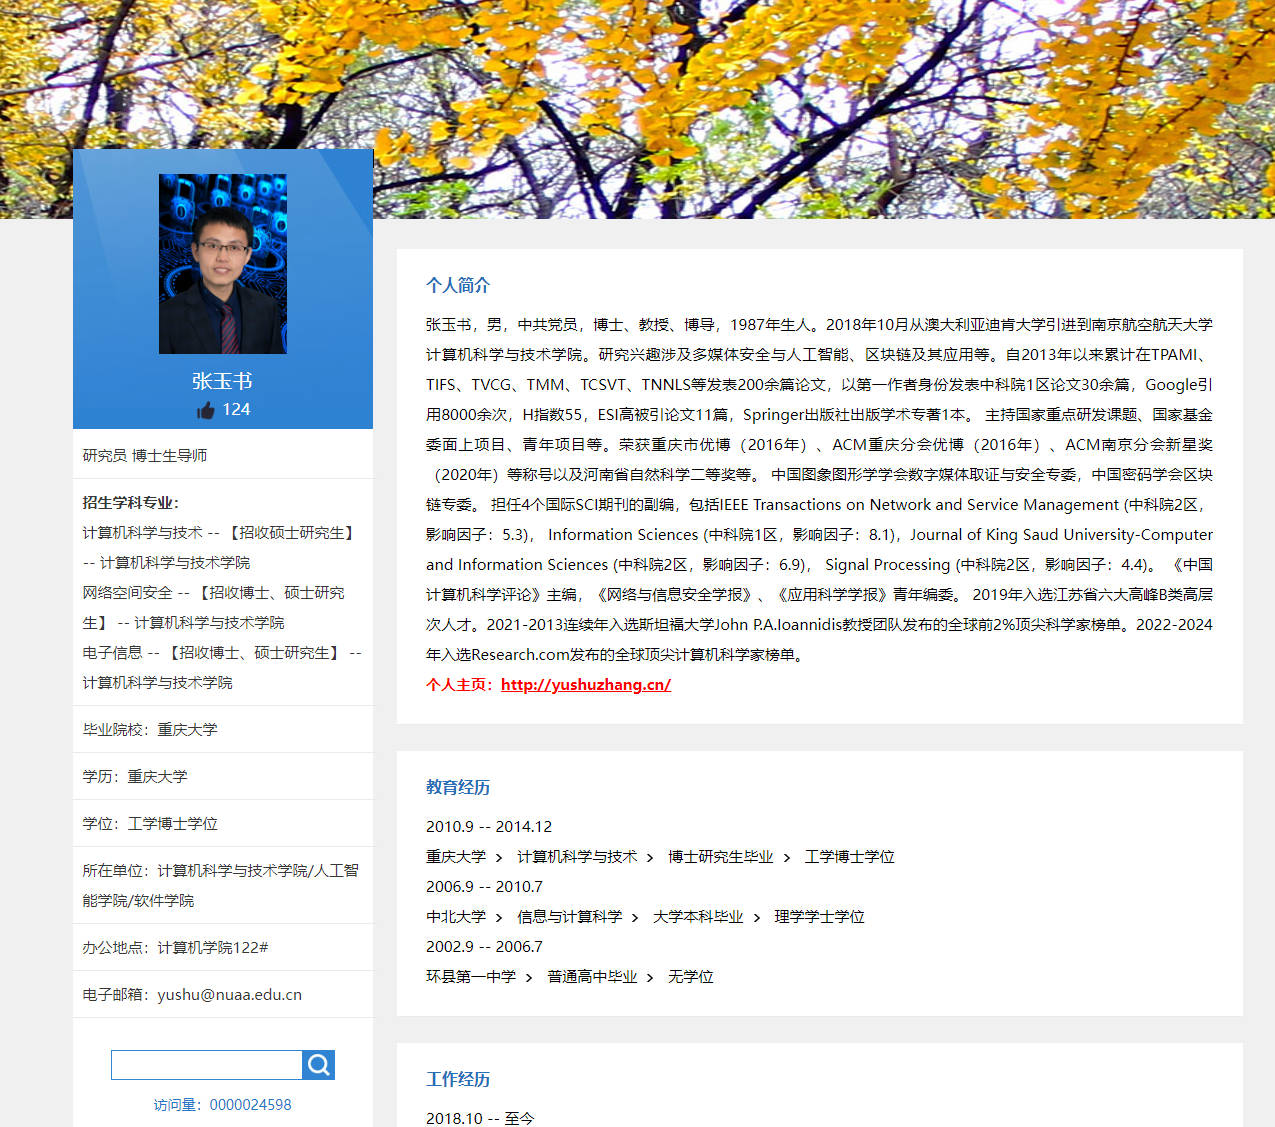
\includegraphics [height=0.17\textheight]{figs/yushu_zhang2.jpg}
    }
    \subfigure [张玉书教授个人主页\cite{yushuzhang3:online}]{\label{fig_yushuzhang3}
    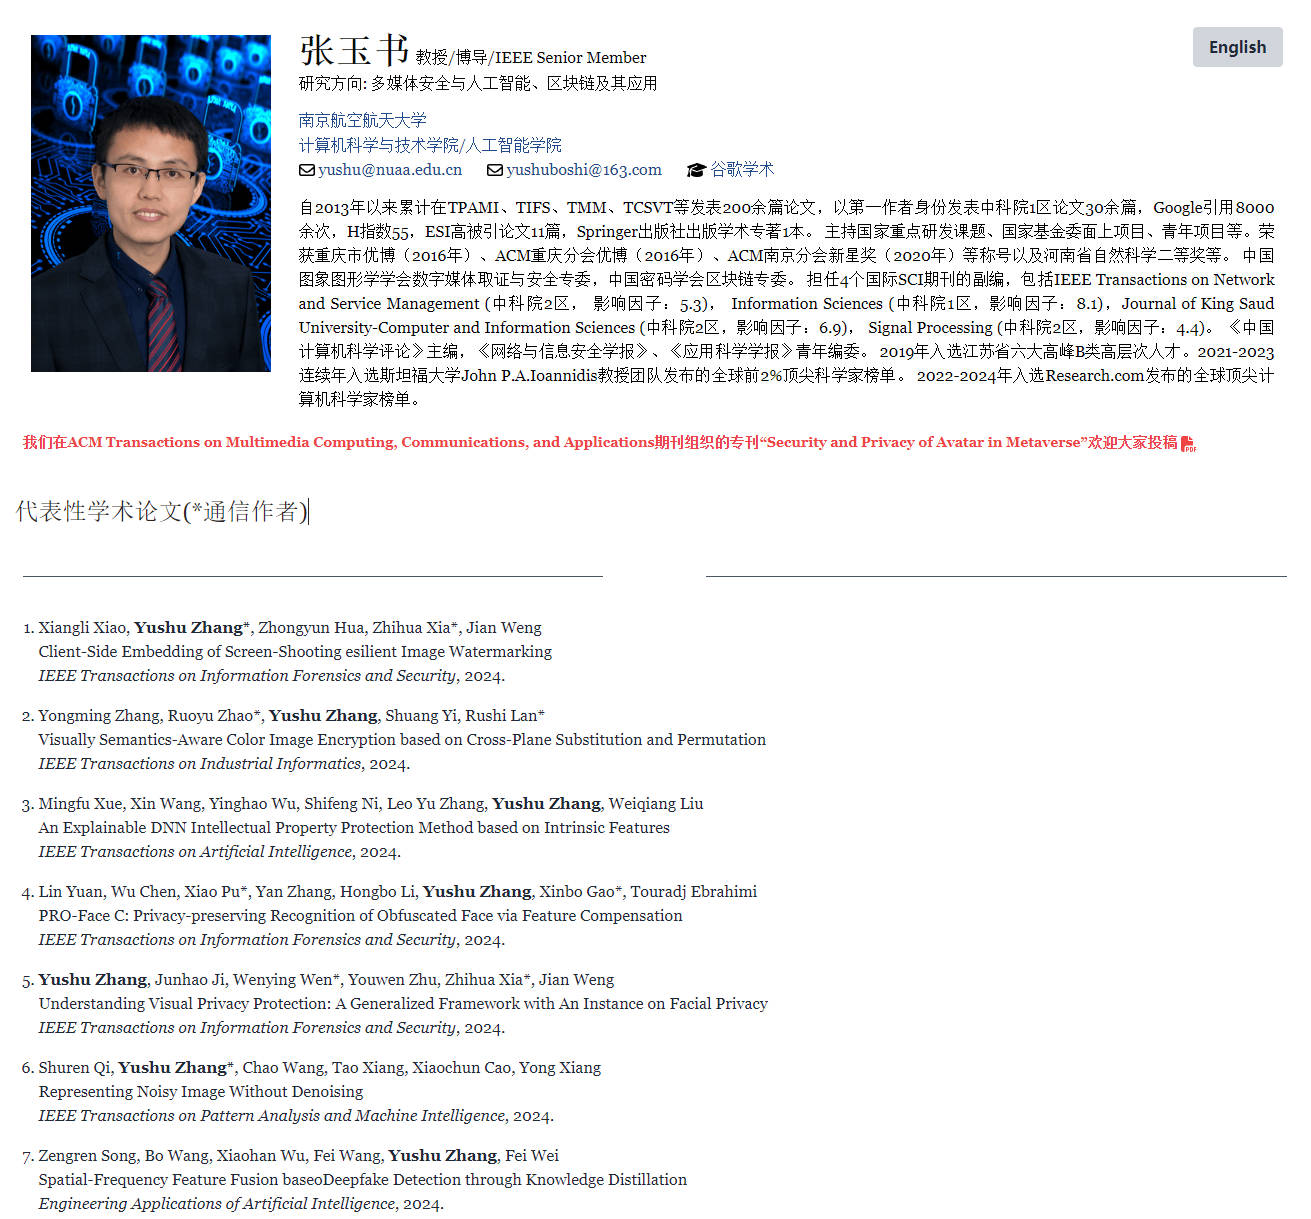
\includegraphics [height=0.17\textheight]{figs/yushu_zhang3.jpg}
    }
    \caption {张玉书教授个人介绍}
\end{figure}

其次介绍该讲座的流程。该讲座从AIGC的概念入手,深入浅出的介绍了生成式数据隐私的隐私性、可控性、真实性与合规性。本次讲座首先普及了基础知识,即什么是AIGC以及AIGC的发展流程。其次科普了AIGC当前面临的数据安全问题,并从生成式数据的隐私性、可控性、真实性、合规性四个角度考量了当前AIGC隐私保护问题的研究成果。最后以总结的形式分享了当前AIGC安全领域依旧可能存在的问题与研究方向。

整个讲座在不失专业性的前提下,以介绍基础内容为切入点,结合当前相关领域研究的最新进展,向观众提供了清晰的思路与高度凝练的综述信息,为想要深入研究的相关从业者提供了快速入门的契机。

\section{引言}

生成式人工智能(AIGC),即由人工智能生成的内容,正迅速发展并广泛应用于各个领域,如自然语言处理、计算机视觉和音频生成等。这项技术不仅能够生成高质量的文本和图像,还能在许多实际应用中提升生产效率和用户体验。例如,OpenAI\cite{OpenAI66:online} 的 GPT-4 能够生成高质量的文章和对话,帮助用户完成写作、翻译和自动摘要等任务;在图像生成领域,如 Midjourney\cite{Midjourn42:online} 和 DALL-E 2\cite{DALLE2O26:online} 等模型可以生成逼真的图像,用于艺术创作、广告设计和娱乐等行业;在音频生成方面,AIGC 技术可以用来生成音乐、语音和音效,应用于媒体制作和个性化服务中。

然而,随着AIGC技术的不断进步,随之而来的安全与隐私问题也逐渐显现,引发了广泛关注。例如,生成式语言模型可能无意间生成包含个人隐私信息的文本,图像生成模型可能侵犯个人肖像权。在社交媒体和新闻领域,生成式模型生成的虚假信息可能误导公众,造成社会恐慌。此外,生成式数据中还可能包含有害或虚假的信息,这些问题在某些情况下可能会被恶意利用,导致严重后果。例如,Deepfake 技术可以生成高度逼真的伪造视频和音频,可能被用来进行网络欺诈和名誉损害。

本报告是对张玉书教授在南京信息工程大学计算机学院、网络空间安全学院所作讲座的整理,旨在探讨生成式数据的安全与隐私问题。张玉书教授在讲座中深入分析了生成式数据的隐私泄露、合规性和合法性等问题,提出了当前面临的主要挑战,并探讨了可能的解决方案。这些讨论涵盖了生成式数据的内生隐私问题、可控性、真实性和合规性等方面。通过这些分析,旨在为相关领域的研究和实践提供参考,推动生成式人工智能技术在确保安全与隐私的前提下健康发展。

例如,为了防止生成式模型生成包含个人隐私的信息,研究者们提出了“模型遗忘”技术,以确保生成模型在训练过程中不会记住敏感数据。此外,针对图像生成模型可能侵犯肖像权的问题,提出了利用扰动和水印技术来保护图像版权和隐私。为了检测和防范生成式数据中的有害信息,研究者们开发了多种生成式检测和归因方法,以确保生成数据的真实性和合规性。

本报告的内容主要来源于张玉书教授的讲座,并结合了相关领域的最新研究进展。希望通过这份报告,能够引起更多研究者和从业者对生成式数据安全与隐私问题的关注,共同探索解决这些问题的方法,确保AIGC技术能够更好地服务于社会。

\section{AIGC的概念}

AI-Generated Content(AIGC)是指由人工智能生成的内容。这些内容包括文本、图像、音频、视频等,涵盖了广泛的应用领域。AIGC的发展伴随着人工智能技术的进步,可以分为以下几个阶段:

\subsection{早期萌芽阶段}

在早期萌芽阶段(20 世纪 50 年代到 90 年代中期),人工智能技术刚刚起步,研究主要集中在理论探索和初步实验上。生成式人工智能的概念逐渐形成,但由于计算能力和数据的限制,其应用还非常有限。例如1966年Joseph Weizenbaum 开发了第一个聊天机器人 ELIZA\cite{ELIZAWik55:online},其通过关键字扫描与重组完成任务,这标志着自然语言处理领域的早期尝试。80年代中期,IBM基于隐形马尔科夫链模型(Hidden Markov Model, HMM)\cite{eddy1996hidden}创造了语音控制打字机Tangora\cite{AlbertTa6:online},该打字机能处理大概20000个单词。80年代末到90年代中,由于高昂的系统成本无法带来可观的商业变现,各国政府纷纷减少了在人工智能的投入,AIGC没有取得重大突破。


\subsection{沉淀积累期}

在沉淀积累期(20 世纪 90 年代中期到 21 世纪 10 年代中期),随着计算机技术的进步和互联网的普及,数据量和计算能力大幅增加,推动了生成式人工智能技术的发展。机器学习和深度学习算法逐渐成熟,为AIGC奠定了基础。如2006年,Geoffrey Hinton 等人提出深度信念网络(Deep Belief Networks)\cite{hinton2009deep},开启了深度学习的研究热潮。2014年,Ian Goodfellow 提出了生成对抗网络(GANs)\cite{goodfellow2020generative},极大地推动了生成式模型的发展。

\subsection{快速发展期}

进入21世纪10年代中期,人工智能技术迎来了爆发式增长,目前增长趋势依旧较高。深度学习算法和大规模数据集的结合,使得生成式人工智能技术迅速进步,逐渐走向实用化。2018年,OpenAI\cite{OpenAI66:online}发布了GPT(Generative Pre-trained Transformer)模型,实现了高质量的文本生成。此后,GPT-2和GPT-3的推出进一步提升了文本生成的质量和应用范围。与此同时,图像生成领域也取得了重大突破,例如DeepMind的DALL-E\cite{DALLE2O26:online}和Midjourney\cite{Midjourn42:online},这些模型能够生成高逼真的图像,应用于艺术创作、设计等多个领域。

在文本生成领域,OpenAI 的 GPT-4 模型能够生成高质量的文章和对话,广泛应用于写作辅助、自动摘要、翻译等领域。例如,自动新闻生成系统可以根据输入的关键词或事件生成完整的新闻报道,提高新闻编辑的效率。

在图像生成领域,Midjourney\cite{Midjourn42:online} 和 DALL-E 2\cite{DALLE2O26:online} 等模型可以生成高质量的图像,被广泛应用于艺术创作、广告设计和娱乐行业。例如,广告公司可以利用这些生成模型快速生成创意图像,以满足不同客户的需求。图\ref{fig_dalle2}、\ref{fig_midjourney}、\ref{fig_stablediffusion}分别展示了使用dalle-2\cite{DALLE2O26:online}、MidJourney\cite{Midjourn42:online}以及Stable Diffusion\cite{CompViss98:online}生成的图像结果。

AIGC 技术在音频生成方面也有显著应用,如生成音乐、语音和音效。例如,Spotify\cite{SpotifyW96:online} 使用生成式人工智能为用户推荐个性化音乐播放列表,而游戏开发公司则利用生成式模型创造逼真的音效和背景音乐。

\begin{figure}[htbp]
    \center
    \subfigure [DALLE\cite{DALLE2O26:online}]{\label{fig_dalle2}
    
\includegraphics [width=0.2\textwidth]{figs/dalle2.jpg}
    }
    \subfigure [MidJourney\cite{Midjourn42:online}]{\label{fig_midjourney}
    
\includegraphics [width=0.2\textwidth]{figs/midjourney.jpg}
    }
    \subfigure [Stable Diffusion\cite{CompViss98:online}]{\label{fig_stablediffusion}
    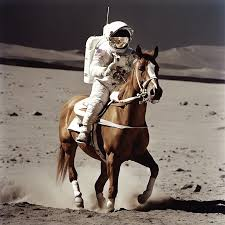
\includegraphics [width=0.2\textwidth]{figs/stablediffusion.jpg}
    }
    \subfigure [DiffSinger\cite{aimusic21:online}]{\label{fig_aimusic}
    
\includegraphics [width=0.2\textwidth]{figs/aimusic2.png}
    }
    \caption {一些著名的AIGC模型与对应的生成结果}\label{fig:eof_12}
\end{figure}

AIGC 技术的发展不仅提升了生产效率,还丰富了用户体验。然而,伴随而来的安全与隐私问题也不容忽视,亟需研究和解决。这些技术的不断进步为我们带来了前所未有的机遇,同时也提出了新的挑战。在推动生成式人工智能技术发展的同时,确保其安全与隐私是我们必须面对的重要课题。

\section{生成式数据的安全与隐私问题}

生成式数据技术在带来巨大便利的同时,也引发了诸多隐私和安全问题,这些问题对技术的广泛应用和社会接受度提出了严峻挑战。生成式语言模型(如GPT-3和GPT-4)和生成式图像模型(如DALL-E和Midjourney)在生成内容时,可能无意间暴露用户的个人隐私信息。

例如,语言模型在处理和生成文本时,可能会泄露用户的个人数据,如姓名、住址、电话号码等敏感信息。这种情况尤其可能发生在模型从包含个人数据的大规模文本数据集训练而来时。用户在与聊天机器人交互过程中,可能无意中提供了敏感信息,而这些信息可能在未来的对话中被模型不恰当地引用或重现。

利用图像生成模型生成的图像可能会侵犯个人肖像权。例如,Deepfake技术可以生成高度逼真的伪造视频和图像,可能被用于恶意用途,如网络欺诈、名誉损害等。如下图\ref{fig_trump}中,网友出于搞笑目的制作了视频“如果中国算发展中国家,那美国也是发展中国家”。尽管这个视频是出于搞笑目的创作的,但如果被有心人士拿去欺骗不知详情的群众,则可能造成严重后果。再如下图\ref{fig_zhapian}中,已有诈骗团伙利用AI生成受害人的熟人生成,以语音的方式取得信任,从而实施诈骗。这不仅侵犯了个人的隐私权,还可能造成社会动荡、财产与心理伤害。

\begin{figure}[htbp]
    \center
    \subfigure [AI美国总统流利用中文表达\cite{aitrump25:online}]{\label{fig_trump}
    
\includegraphics [width=0.45\textwidth]{figs/aitrump.jpg}
    }
    \subfigure [新型AI诈骗\cite{AI68:online}]{\label{fig_zhapian}
    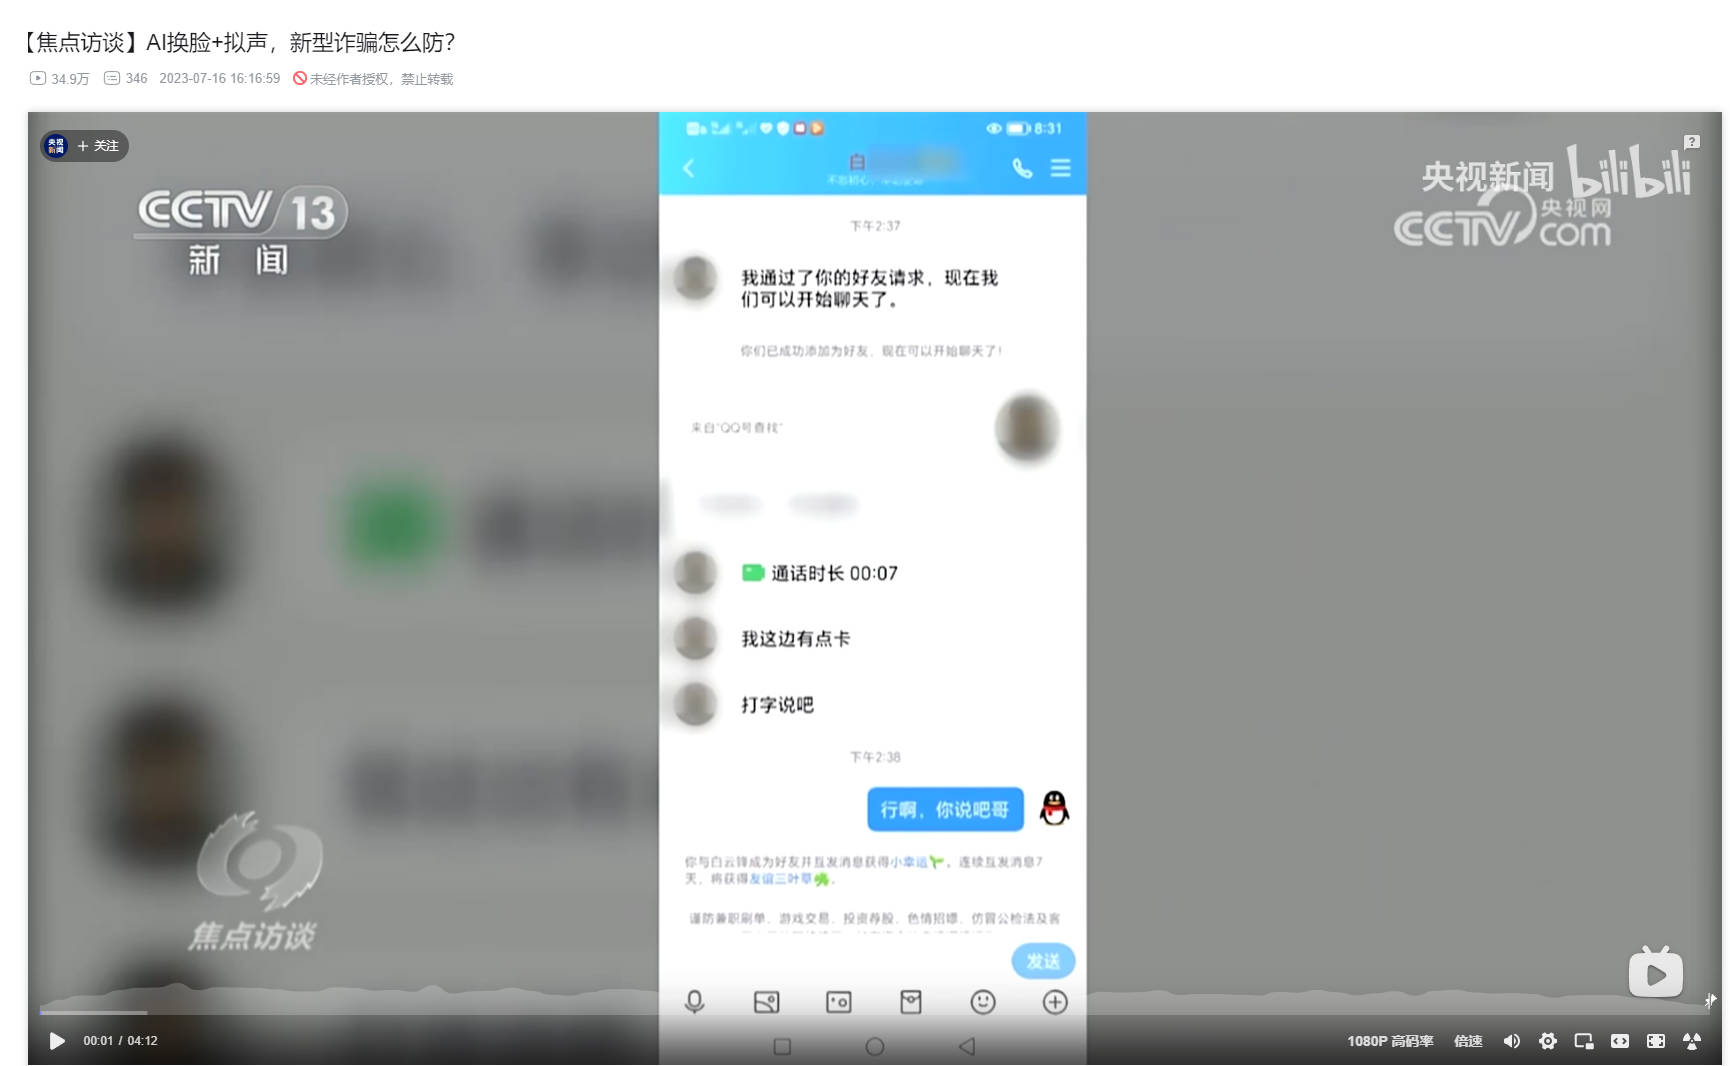
\includegraphics [width=0.45\textwidth]{figs/aizhapian.jpg}
    }

\end{figure}

生成式数据在合规性和合法性方面也面临诸多挑战。生成式模型可能生成包含有害内容的数据,例如仇恨言论、色情内容、虚假信息等。这些毒性内容不仅违反法律法规,还可能对社会造成负面影响,增加社会不稳定因素。生成式模型有时会生成虚假的或不准确的信息,这在新闻报道、社交媒体等领域尤其危险。反事实内容可能误导公众,造成错误的认知和决策,甚至引发社会恐慌。例如,自动化新闻生成系统可能在未经过充分验证的情况下发布虚假新闻,导致公众恐慌。

在讨论生成式数据的安全问题时,不应仅关注生成模型,还应关注生成数据流程中的其他环节,如数据收集和数据处理过程。用于训练生成式模型的数据集可能存在隐私和版权问题。许多数据集在未经用户明确同意的情况下收集用户数据,这可能侵犯用户隐私权。此外,数据集中可能包含受版权保护的内容,未经授权的使用可能引发法律纠纷。数据在处理和存储过程中也可能面临泄露风险。例如,数据在传输过程中可能被截获,存储在云端的敏感数据可能面临黑客攻击的风险。数据的匿名化和去标识化处理不当,也可能导致隐私泄露。

生成数据的流程涉及多个环节,每个环节都有可能引发安全和隐私问题。在数据收集阶段,大量用于训练生成模型的数据可能来自公开互联网,这些数据未经筛选,可能包含敏感信息或不当内容。而在预处理过程中,如果未对数据进行充分的清洗和去标识化处理,可能导致隐私泄露。训练过程中,如果未采用适当的隐私保护技术(如差分隐私),可能导致训练数据中的敏感信息泄露。最后,生成的数据在发布前应经过严格审查,以确保不包含敏感信息或有害内容。

为了应对这些问题,研究者们提出了多种解决方案。例如,差分隐私技术可以在模型训练过程中保护数据隐私,数据水印技术可以在生成数据中嵌入识别标识,以追踪和防止滥用。此外,政策和法规的制定也至关重要,通过法律手段规范生成式数据的收集、处理和使用过程,可以在一定程度上保障数据安全和用户隐私。

下面将从生成式数据的隐私性、可控性、真实性与合规性角度介绍部分生成式数据安全的相关工作。

\subsection{生成式数据的隐私性}

在处理生成式数据的隐私性方面,目前的工作围绕两个方面展开。其一为AIGC内生隐私,该工作以优化生成式人工智能模型为主要目标,以确保生成式人工智能模型中不出现可能的隐私泄露问题;其二为AIGC助力隐私,该工作以利用生成式数据技术来增强隐私保护为主要目标。

\subsubsection{AIGC内生隐私}

生成式数据模型在训练过程中,往往需要大量的真实数据。这些数据中的分布和模式可能会在生成数据中复现,导致隐私泄露。

生成式模型有时会记住训练数据中的具体细节,并在生成内容时无意中复现这些细节。如果生成的数据包含敏感信息,如个人身份信息、地址或其他私密数据,则应立即丢弃这些生成内容,并对模型进行调整或重新训练,以确保敏感信息不会再次被生成。

在构建和使用数据集时,如果发现数据集中包含隐私敏感的信息,则应尽量减少使用这些数据,或通过数据去标识化、加密等技术手段对数据进行处理,减少隐私泄露的风险。这包括对个人信息的匿名化处理,删除或模糊化处理敏感信息等。

\subsubsection{AIGC助力隐私}

尽管生成式数据存在隐私风险,但也可以利用生成式数据技术来增强隐私保护。通过修改生成的数据,保护个体隐私。

例如,在人脸识别领域,通过生成式对抗网络(GAN)技术对人脸图像进行修改,可以生成在视觉上不可识别的图像,但保留机器识别所需的特征。这种技术可以用于隐私保护,如在监控视频中对个人进行匿名化处理,既能满足安全监控需求,又能保护个人隐私。

生成式数据还可以用于创建合成数据集,这些数据集在统计上与真实数据类似,但不包含任何真实的个人信息。这种合成数据可以用于训练和测试模型,确保在开发和部署过程中不会泄露真实数据。

\subsection{生成式数据的可控性}

在生成式数据的应用中,如何确保数据的可控性和可追溯性是一个重要的问题。代表性工作包括阻止 GAN 模型对预期生成结果的直接访问与可追溯性的确保。

\subsubsection{阻止直接访问}

为防止生成模型对生成结果的直接控制,可以在生成图像时添加扰动。例如,在GAN生成的图像上添加噪声或水印,使得生成图像在视觉上没有明显变化,但可以有效防止生成模型对结果进行直接操控。这种方法不仅能保护生成数据的安全,还能增强对生成数据的控制能力。

\subsubsection{可追溯性的确保}

生成数据的可追溯性是指可以追溯生成数据的来源和生成过程。通过在生成数据中嵌入水印等技术手段,可以实现对数据的追踪和溯源。例如,基于区块链的水印技术可以为每个生成数据创建唯一标识,确保在数据流通过程中可以随时追踪其来源和修改历史。这种技术虽然投入较大,但在数据安全和隐私保护方面具有较高的保障作用。

\subsection{生成式数据的真实性}

在确保生成式数据真实性方面,目前有两项主要工作。其一为生成式检测,该工作的主要目标为判断某项数据是否为生成式模型生成的;其二为生成式归因,该工作的主要目标是判断某个生成式数据是由哪个生成式模型生成得到的。

\subsubsection{生成式检测}

如何判断数据是否为生成的,这是确保数据真实性的重要环节。主要方法包括伪影检测、误差分析、不变性探索、概率曲率判断、文本分散性等。

\textbf{伪影检测:}基于GAN生成的图像中常存在伪影,通过检测这些伪影可以判断图像是否为生成的。伪影是生成图像中无法完全消除的人工痕迹,通过高级图像分析技术可以识别这些痕迹。

\textbf{误差分析:}通过源模型生成后的图像误差比真实图像小,可以通过分析图像误差来判断其是否为生成的。生成模型在生成图像时,会产生细微的误差模式,这些模式与真实图像不同,通过误差分析可以有效识别生成图像。

\textbf{不变性探索:}真实数据通常具有不变性,例如图像中的自然光影和纹理特征。生成数据可能在这些方面表现出异常,通过探索和分析这些不变性,可以有效区分生成数据和真实数据。

\textbf{概率曲率判断:}生成数据的概率分布曲率与真实数据有所不同,通过分析概率分布曲率,可以识别生成数据。生成模型在生成数据时,通常会形成特定的概率分布模式,通过曲率分析可以有效检测生成数据。

\textbf{文本分散性:}人类的文字表达通常更为发散,而机器生成的文字较为集中。通过分析文本的分散性和聚合性,可以判断文本是否为生成的。例如,生成文本往往在词汇和句式上表现出较高的重复性,通过自然语言处理技术可以识别这些特征。


\subsubsection{生成式归因}

判断数据是由哪种模型生成的,是确保数据真实性和溯源的重要步骤。主要方法包括模型指纹识别、概念归因等。

\textbf{模型指纹识别:}
不同扩散模型具有不同的指纹,通过构建多分类器来识别这些指纹,可以区分出数据是由哪种模型生成的。模型指纹是生成模型在生成数据时留下的独特痕迹,通过高级算法分析可以识别这些痕迹。


\textbf{概念归因:}
将生成图像归因于其训练数据的概念,如风格、艺术家等。例如,通过分析图像的风格特征,可以判断其是由哪种生成模型生成的。这种方法可以帮助追溯生成数据的来源,并确保数据的真实性和版权保护。

\subsection{生成式数据的合规性}

当我们提及生成式数据的合规性时,一般是在说其无毒性与事实性。

\subsubsection{无毒性}

无毒性是指生成的数据不包含有害或不当内容。这些有害内容可能包括仇恨言论、色情内容、虚假信息、暴力描述等。确保生成安全数据的关键在于无毒的训练数据集。一些研究专注于此方面,致力于引导模型不生成有毒数据。

\textbf{数据集清洗:}对训练数据集进行清理是一种确保无毒性的有效方式。通过对训练数据集进行严格的筛选和清理,剔除其中的有害内容,如仇恨言论、色情内容和虚假信息等。这可以有效降低生成模型生成有毒数据的风险。

\textbf{模型优化:}对模型进行优化也是一种较为流行的方式。通过对生成模型进行优化,使其在生成数据时能够自动识别并过滤有害内容。例如,使用对抗性训练方法,可以使模型在生成过程中更具安全性和合规性。

\subsubsection{事实性}

事实性是指生成的数据应符合客观事实和真实情况。确保生成数据的事实性对于其可信度和可靠性至关重要,特别是在新闻报道、科学研究和法律文书等应用场景中。生成数据的事实性是确保其可信度和可靠性的重要因素。

\textbf{多模型辩论:}对于用户提问,可以使用多个自动对话机器人进行辩论,统一结论后再反馈给用户。这种方法通过引入不同观点和分析,提高生成数据的准确性和可靠性。

\textbf{事实性验证:}开发基于事实的验证系统,对生成数据进行验证和校准。例如,通过引入外部数据库和知识图谱,可以对生成数据进行实时验证,确保其内容的准确性和事实性。

通过综合考虑和解决上述生成式数据技术面临的这四个关键问题,可以提高生成式数据的安全性、可靠性和社会接受度,推动生成式人工智能技术的健康发展。

\section{总结}

尽管当前AIGC安全与隐私问题正引起广泛的关注,但当前依旧有不少可以改进的部分,以下是一些可能的研究方向。
\begin{enumerate}
    \item 可证明的机器/概念遗忘:尽管有实验表明机器可能会遗忘,但如何证明这一点?
    \item 生成式数据的篡改检测:生成式数据可能遭受恶意篡改,检测篡改较为困难。
    \item 基于真实数据不变性的生成式检测:现有的生成式检测关注生成数据的变量,但真实数据的分布具有稳定性,可以基于此做检测。
    \item 隐藏毒性的检测:攻击者可能通过生成式数据隐藏有毒信息,难以察觉。
    \item 合规性的机器评估:尽管目前有评估方法,但仍需进一步研究如何机器评估生成式数据的合规性。
\end{enumerate}
%%%%%%%%%% 参考文献 %%%%%%%%%%

%%%%%%%%%% 参考文献 %%%%%%%%%%
\bibliography{bibliography}
%%%%%%%%%% 附录(可选) %%%%%%%%%%

%%%%%%%%%% 附录(可选) %%%%%%%%%%



\end{document}
